\documentclass{article}

\author{Nicol\'o Ruggeri}
\title{Combinatorial Optimization Final Report}
\date{\null}

\usepackage{amsmath}
\usepackage{amsfonts}
\usepackage{hyperref}
\hypersetup{
     colorlinks = true,
     linkcolor = blue,
     anchorcolor = blue,
     citecolor = blue,
     filecolor = blue,
     urlcolor = blue
     }
     
\usepackage{graphicx}

\usepackage[procnames]{listings}
\usepackage{color}

\usepackage{booktabs}




\begin{document}
% -------------------------------------------
% stuff for Python code in document
\definecolor{keywords}{RGB}{255,0,90}
\definecolor{comments}{RGB}{0,0,113}
\definecolor{red}{RGB}{160,0,0}
\definecolor{green}{RGB}{0,150,0}
 
\lstset{language=Python, 
        basicstyle=\ttfamily\small, 
        keywordstyle=\color{keywords},
        commentstyle=\color{comments},
        stringstyle=\color{red},
        showstringspaces=false,
        identifierstyle=\color{green},
        procnamekeys={def,class}}
        
% --------------------------------------------


\maketitle

\section{Introduction and  First Notations}
In this report we analyze the performances of two different methods for solving a particular instance of the TSP problem. Specifically, we solve the problem presented below with a linear programming network flow formulation, as requested in homework 1, and with a genetic algorithm presented in section \ref{sec:algorithm}. \\
In our case we formulate the problem on a complete graph $G = (V, E)$ where the adjacency matrix $A \in \mathbb{R}^{|V|}$ of $G$ is symmetric and dense. In our case we consider a weighted graph, so that $a_{i,j} \in \mathbb{R}_{\ge 0}$ is the cost of moving from point $j$ to $i$. We will explain how these distances are generated in section \ref{sec:data}.\\
The particular properties of the matrix reflect two assumptions that we make on our model, namely:
\begin{itemize}
\item $A$ symmetric. This means that the cost of going from $j$ to $i$ is the same as going the other way around. This makes sense for the underlying practical problem at hand, i.e. the one of a drill moving from position $i$ to $j$
\item $A$ dense (and in the particular case of our experiments, with almost all elements strictly positive, see sections \ref{sec:data} and \ref{sec:experiments}). With a slight abuse of terminology, here we mean that all entries of $A$ are available (or, equivalently for the problem, lesser than infinite). This reflects the fact that $ij \in E \hspace{2mm} \forall i, j$, i.e. the drill can move between any two arbitrary points
\end{itemize}
In the following section we will refer to points equivalently as nodes, and to the connections between them as edges (from the graph formulation).


\section{Data Generation}\label{sec:data}
\subsection{Distance Matrix}
We frame the problem as that of moving between points in the unitary square $[0, 1]^2$. Notice that this doesn't represent a restriction, since it can be seen as a rescaling of a problem of any size. Given that we have a finite number of points, we can number them from $1$ to $n$, so that the vertex set of the graph is $V = \{ 1, \ldots, n  \}$. Now we consider these two dimensional sampled vectors $x_i \in [0, 1]^2 $, that represent the position of every point in the drilling board. If we want to generate the cost matrix $A$ from these points, a natural interpretation could be to assume a movement time proportional to the distance between the points. In fact in the experiments section \ref{sec:experiments} we consider a distance matrix given by
\begin{equation}\label{eq:cost}
a_{ij} := {|| x_i - x_j ||}_2
\end{equation} 
The choice of the 2-norm is arbitrary, and could be replaced by any euclidean norm, which could in principle affect the final optimal solution. \\
Notice that this approach is easily generalized in many ways. For example to exclude some edges from the final solution we just need to impose $a_{ij} = +\infty$. To differenciate the cost between points we can substitute the formulation above with $a_{ij} = f(x_i, x_j)$ for some function $f$ (that doesn't even need to be symmetric in the arguments, as the genetic algorithm from section \ref{sec:algorithm} and the OPL solver accept totally general distances).  

\subsection{Experimental Data}\label{sec:experimental_data}
Following the process above, we just need to generate any number $n$ of points $x_i \in [0, 1]^2 $, and then build the cost matrix that we will input to the solvers. In our case we decided to generate these points at random in the following way:
\begin{itemize}
\item a number $n_1$ of points is generated according to a mixture of equiprobable two-dimensional gaussians with given variance $\sigma^2$ and means $\mu_1, \ldots, \mu_k$. Since the sampled points could end up being outside the allowed space, we clip all the points' coordinates in $[0, 1]$. 
\item the remaining $n-n_1$ points are radomly distributed on a fixed granularity grid on  $[0, 1]^2$. This allows to have some clusters, given by the gaussians, and some other points scattered on the square. 
\end{itemize}
Notice that this procedure allows, with small probability, overlapping points. This is not a problem for our model, as the solvers need to be able to recognize this peculiarity and find a solution where such points are visited sequentially, since this movement has cost 0 according to equation \eqref{eq:cost}. \\
This particular choice of data generation has been made to resemble the actual real life problem at hand: the drill is moving over an electric board making holes in preparation for its use. By looking at an actual finished electric board (figure \ref{fig:board}) we can see that some points are naturally clustered together for certain electric components, and some other are less close one another and more distributed.

\begin{figure}
\centering
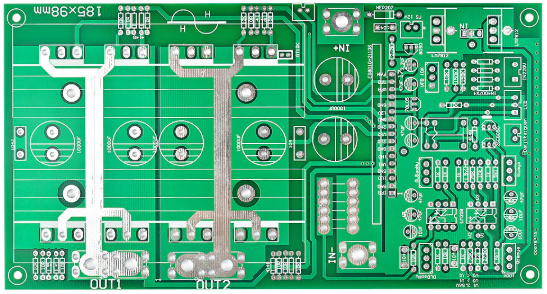
\includegraphics[width=0.5\textwidth]{pics/electric_frame.png}
\caption{An electrical component. Notice the presence of clustered components, as well as scattered points}
\label{fig:board}
\end{figure}


\section{The Genetic Algorithm}\label{sec:algorithm}
After the use of the OPL model for homework 1, we decided to implement a heuristic for the solution of the problem described above in homework 2. Specifically, we designed a genetic algorithm, represented as a class \textit{TSPSolver} in the code attached to this report. Moreover, we decided to implement this class from scratch. This choice is not due to the lack of Python libraries for genetic algorithms (see for example \href{https://deap.readthedocs.io/en/master/}{DEAP} or  \href{https://pyeasyga.readthedocs.io/en/latest/index.html}{pyeasyga}), but rather to a will to better understand the challenges of a complete implementation of a model, as well as to a undoubtedly enhanced learning experience. \\
Details about the implementation are included in the following section.

\subsection{Implementation Details}
\subsubsection{Functionalities}
The genetic algorithm represents solutions to the TSP problem using the path representation. This means that a solution is a permutation of $\{0, \ldots, n-1\}$ where the nodes are listed in order of visit. The only neighbourhood considered is the standard 2-opt neighbourhood. \\
The following options have been made available in the implementation (see code attached for further details, it has been made as clear and documented as possible):
\begin{itemize}
\item \textbf{initialization}: individuals (i.e. solutions) are initialized at random. Every generation is made up of a customized size of individuals. At initialization time it is possible to choose a fraction of individuals to substitute with their best 2-opt neighbour

\item \textbf{selection of individuals}: all selection types seen in class have been made available, namely montecarlo, linear ranking and $n$-tournament. This selection type affects which individuals are chosen for mating.

\item \textbf{mating}: two types of mating have been made available. The first is the selection of a given number of pairs of individuals. Every pair gives rise, according to the type of crossover, to one of two individuals as offspring. The second is the selection of a "mating pool": a number of individuals is chosen, and every possible couple undergoes crossover.

\item \textbf{crossover}: many types of crossover are available in literature, two possible reviews are \cite{gupta2011study} and \cite{abdoun2012comparative}. Since we found more clarity in the explanations from \cite{gupta2011study}, we implemented all the crossover types presented there. For clarity, we stick to the notation in reference in the code (which is also pretty intuitive, see the private method of the solver \textit{TSPSolver.\_crossover})

\item \textbf{mutation}: with a customized probability, every new individual undergoes mutation. If mutated, every individual is substitued with a random 2-opt neighbour

\item \textbf{generation replacement}: it is possible to keep the best $m$ individuals among the old and new generation, or to remove the worst $m$

\item \textbf{stopping criterion}: there are some stopping criteria available: the maximum number of non improving evolution steps, the time limit, the target score (i.e. stop as soon as the best individual passes a certain score threshold) and the maximum number of generations. These can also be used in combination.

\item \textbf{fitness function}: here we allowed no option but the total cost of the path (including the return to the initial node 0). This point is just to highlight that for efficiency recursive evaluation of the fitness score has been used when possible (i.e for all points from the second generation onward)
\end{itemize}
As a final remark, we would like to to underline that the code has been factorized as much as possible, building appropriate private (or public, even though the difference is almost non-existent in Python) methods for \textit{TSPSolver}. This allows modification/integration of everyone of these customizations with relative ease. The code is also available on \href{https://github.com/NRuggeriProjects/Combinatorial-Optimization}{my GitHub account}.


\subsubsection{Technical Details}
In this section we just include some technical details about the implementations itself. \\
As we said, the solution representation of choice is the path representation. Since the natural translation is to use array objects to encode such solutions (or individuals), in Python one could use, for example, a simple list. We decided to go for \href{https://www.numpy.org/}{numpy} arrays. These allow for optimized vectorial operations, which come in handy at the crossover step, and are usually regarded as an efficient array tool for general use. \\
The actual solution flow executes as follows. 
\paragraph*{Initialization} First, a \textit{TSPSolver} instance needs to be created. At initialization moment the solver object is endowed with some attributes regarding the options included in the section above. At this stage also some other placeholder attributes are attached to the it. These include some private attributes, used for the solution loop (such as the starting time in case the time is among the sopping criteria, the generations count, etc.) as well as variables that are inferred when an actual cost matrix is given as input for the problem. \\
The private attibutes (which are indicated by a leading underscore in Python) are used by the solver and are not intended for the final user. These inlcude the current generations and relative fitness values, and are continuously modified during the "evolution" step. Second, there are variables intended for posterior reference, such as the best individual (i.e. the solution) and the relative fitness. Also the cost matrix and problem size are public attributes that one can access later. 
\paragraph*{Solution} After a solver object has been created, one can call the \textit{solve} method, providing a cost matrix. Notice again, that the cost matrix has to be a square, two-dimensional, numpy array. This \textit{solve} method is actually just a coordinator that, after saving all the variables from above (cost matrix, problem size, etc.) sequentially calls private methods for the single steps of the evolution. These are \textit{\_initialize\_generation} and, while no stopping criterion is satisfied, \textit{\_evolve\_generation}. The \textit{\_evolve\_generation} method, in turn, calls in order the \textit{\_select\_individuals} and \textit{\_mating\_and\_mutation} and then updates the actual generation according to the generation replacement criterion provided by the user. \\
In the end, the code for running the solution loop is pretty simple, and looks something like this:
\newline
\begin{lstlisting}	
solver = TSPSolver()     # in case modify default parameters

with open('cost_matrix.pkl', 'rb') as file:
	cost_matrix = pkl.load(file)
	
solver.solve(cost_matrix)

print(
'The best solution found is {}, with score {}'.format(
	solver.best_individual, solver.best_fitness
	)
)
\end{lstlisting}
Notice that this way of handling problems, i.e. by using a class that stores all the information needed for and after the solution is also typical of the Python approach to machine learning, for example in \href{https://scikit-learn.org/stable/}{scikit-learn} objects or \href{https://keras.io/}{keras} models. The advantage is the possibility of clear and concise sintax, automation and possibility of simple saving procedures, since the class instance incapsulates all the parameters and procedures.

\subsection{Implementation Challenges}
One of the main reasons for the usage of genetic algorithms is their relative speed and ease of implementation. We found that this is actually true, with just some caveats. The implementation of the single parts of the algorithm is not very challenging, especially due to the fact that the procedure is well organized into distinct sections (selection, mating, crossover, etc.) and due to the (in this case) very clear and explicative metaphor with population evolution. One downside, though, is that in the moment in which one wants to allow more options, things could get messy. For this reason we report, as main difficulty encountered, the need to keep every functionality properly organized, mainly by a great deal of code factorization. As we said above, this need has in the end made the code more tidy and organized, with the possibility to add new features with relative ease.




\section{Experiments}\label{sec:experiments}
As requested for the homework, here we present a comparison of the performances of the exact OPL solver, with the network flow formulation, and the genetic algorithm. The datasets are built as follows: following the procedure from section \ref{sec:experimental_data}, we produce three datasets of sizes 20, 100 and 200 nodes. In these, half of the points come from the gaussian mixture, the other half are scattered on a grid. Plots of the data are presented in figure \ref{fig:datasets}.

\begin{figure}
    \centering
    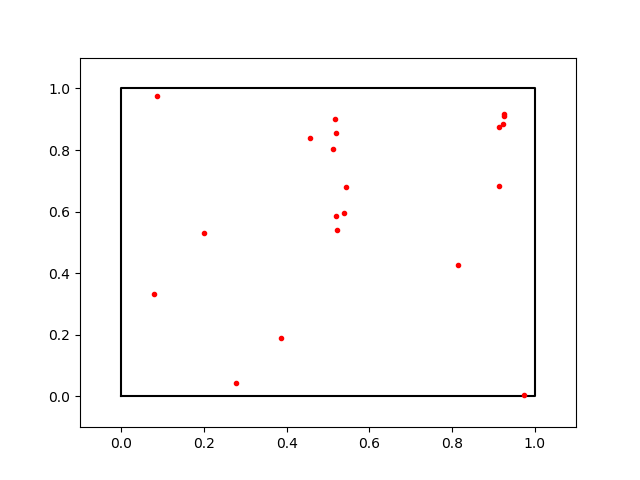
\includegraphics[width=0.3\textwidth]{pics/experimental_data_20.png}
   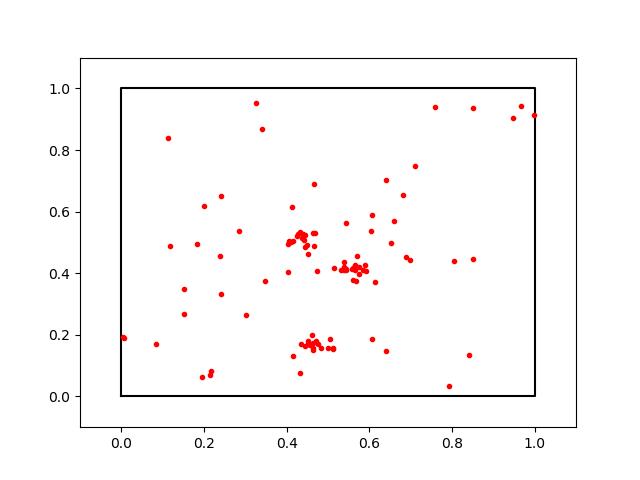
\includegraphics[width=0.3\textwidth]{pics/experimental_data_100.png} 
   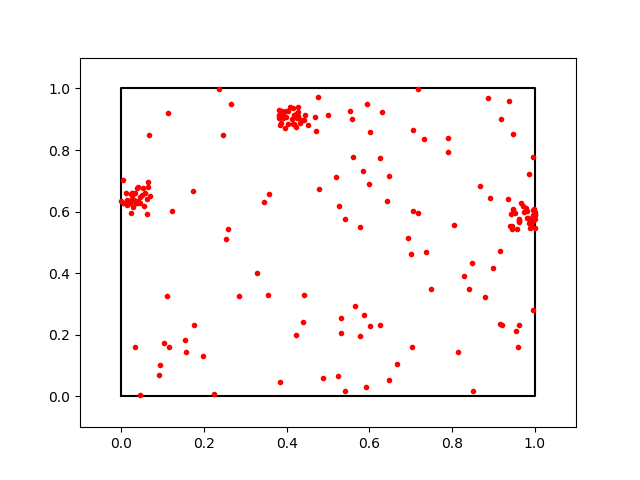
\includegraphics[width=0.3\textwidth]{pics/experimental_data_200.png}
    \caption{synthetic datasets used for the experiments. The sizes are respectively of 20, 100 and 200 nodes. Gaussian clusters points are visible among all other points.}
    \label{fig:datasets}
\end{figure}

\subsection{Parameters Selection}\label{sec: parameters selection}
For everyone of the datasets studied, we first need to run a parameter optimization procedure on the genetic algorithm. The way we chose to do so is to try to solve the specific problem instance on a grid of possible parameters, and then keep the best setting for the experiments. The only difference between the actual experiments and the parameters selection phase is the stopping criterion: to allow for fast exploration of the parameters grid we set a early stopping criterion with respect to the final experiment. Settings for the grid search, including the more strict stopping criteria and the best settings found, are included in table \ref{tab: parameters selection}. \\ \newpage
For all other parameters the default value is used, namely: \\
\newline
\textit{
TSPSolver( \\
\textbf{init\_size}=CUSTOM, \textbf{init\_type}='best2opt', \textbf{init\_best2opt\_frac}=0.2, \\
\textbf{fitness}='total\_cost', \textbf{selection='montecarlo'}, \textbf{mating}='tuples', \\
\textbf{mating\_n}=CUSTOM, \textbf{crossover}='OX', \textbf{mutation\_prob}=CUSTOM,\\
\textbf{gen\_replacement}='keep\_best', \textbf{gen\_replacement\_par}=CUSTOM, \\
\textbf{stopping}=CUSTOM \\
)
}
\newline

\begin{table}[]
\addtolength{\leftskip} {-2cm} % increase (absolute) value if needed
\addtolength{\rightskip}{-2cm}
\begin{tabular}{@{}llll@{}}
                                                                                         & 20 nodes                                                                                           & 100 nodes                                                                                          & 200 nodes                                                                                            \\ \cmidrule(l){2-4} 
\multicolumn{1}{l|}{\begin{tabular}[c]{@{}l@{}}mating\_n \\ (= init\_size)\end{tabular}} & \multicolumn{1}{l|}{50, 100, 150}                                                                  & \multicolumn{1}{l|}{500, 1000, 1500}                                                               & \multicolumn{1}{l|}{2000, 5000, 8000}                                                                \\ \cmidrule(l){2-4} 
\multicolumn{1}{l|}{mutation\_prob}                                                      & \multicolumn{1}{l|}{0.2, 0.4, 0.6}                                                                 & \multicolumn{1}{l|}{0.2, 0.4, 0.6}                                                                 & \multicolumn{1}{l|}{0.2, 0.4, 0.6}                                                                   \\ \cmidrule(l){2-4} 
\multicolumn{1}{l|}{generation size}                                                     & \multicolumn{1}{l|}{50, 100, 150}                                                                  & \multicolumn{1}{l|}{500, 1000, 1500}                                                               & \multicolumn{1}{l|}{2000, 5000, 8000}                                                                \\ \cmidrule(l){2-4} 
\multicolumn{1}{l|}{stopping criteria}                                                   & \multicolumn{1}{l|}{\begin{tabular}[c]{@{}l@{}}time: 100\\ not\_improving\_gen: 1000\end{tabular}} & \multicolumn{1}{l|}{\begin{tabular}[c]{@{}l@{}}time: 100\\ not\_improving\_gen: 1000\end{tabular}} & \multicolumn{1}{l|}{\begin{tabular}[c]{@{}l@{}}time: 1000\\ not\_improving\_gen: 10000\end{tabular}} \\ \cmidrule(l){2-4} 
\multicolumn{1}{l|}{best setting}                                                        & \multicolumn{1}{l|}{150, 0.6, 150}                                                                 & \multicolumn{1}{l|}{1500, 0.6, 1500}                                                               & \multicolumn{1}{l|}{8000, 0.6, 8000}                                                                \\ \cmidrule(l){2-4} 
\end{tabular}
\caption{grid search and relative stopping criteria for the genetic algorithm on the three datasets of size 20, 100 and 200 nodes. The best setting found includes the values of the parameters, in order mating\_n (and init\_size equal), mutation probability and generation size}
\label{tab: parameters selection}
\end{table}

As a side note, we would like to highlight the fact that bayesian optimization techniques could be applied as this problem is suited for extensive hyperparameter tuning (for a review about bayesian optimization, see for example \cite{shahriari2015taking}).

\subsection{Results}
For evaluation, we run the exact solver and the genetic algorithm 5 times each on each of the first two datasets. We just run once on the third one, allowing a longer time limit. This procedure is justified by the fact that the variability in the results from the first two datasets is low enough to show that results are consistent throughout experiments. Consequently we show confidence intervals only in figure \ref{fig:20and100points}, and only for the genetic algorithm, since the exact solver has almost zero variance. \\
Moreover, even if only with 200 points, the OPL solver requires more or less two hours to only find a feasible solution (see figure \ref{fig:200points}), making repeated experiments very time consuming. We comment the results separately in the following sections.

\paragraph*{20 nodes dataset}

\begin{figure}
    \centering
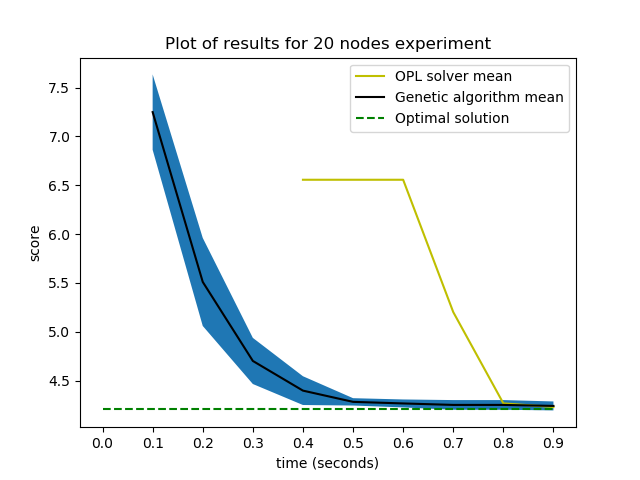
\includegraphics[width=0.4\textwidth]{pics/20_nodes_results.png}
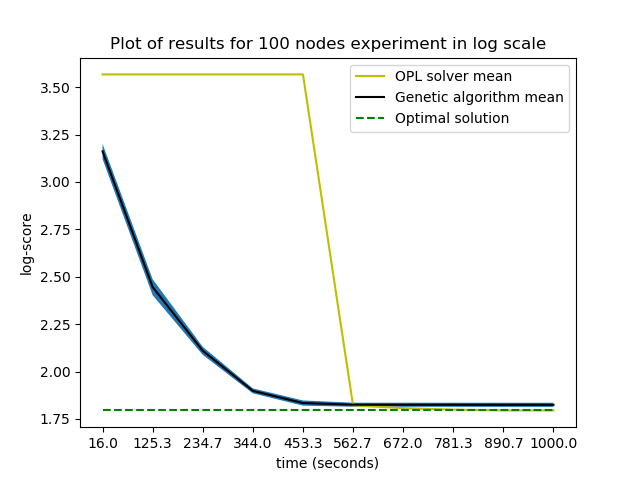
\includegraphics[width=0.4\textwidth]{pics/100_nodes_results.png}
 \caption{results of the experiments of the two smaller datasets of 20 and 100 points}
\label{fig:20and100points}
\end{figure}


Results are presented in figure \ref{fig:20and100points} (left).
For this small instance the exact solution is reached in a short time from the OPL solver. The comparison between the gentic algorithm and the exact solver is interesting, and presents some characteristics that reflect what we usually expect. In fact the genetic algorithm in general finds a generic solution in a shorter time (indeed, it is already provided with a population of feasible solutions at initialization time), and keeps a better solution in time, untill the OPL solver gets close to the optimum.

\paragraph*{100 nodes dataset}
To allow for a fair comparison between the two methods, the same time constraint of 1000 seconds has been applied. As we can see, the size of the population, both at initialization and during evolution, has been increased to comply with the bigger problem size, as from section \ref{sec: parameters selection}. \\
Results are presented in figure \ref{fig:20and100points} (right, notice the log-scale). Even though the OPL solver seems to find a solution on the spot, it then doesn't improve for a very long time. The genetic algorithm instead finds a very good solution in a very short time, which is overcome only after the exact solver approaches (and eventually reaches) the optimal solution.


\paragraph*{200 nodes dataset}

\begin{figure}
    \centering
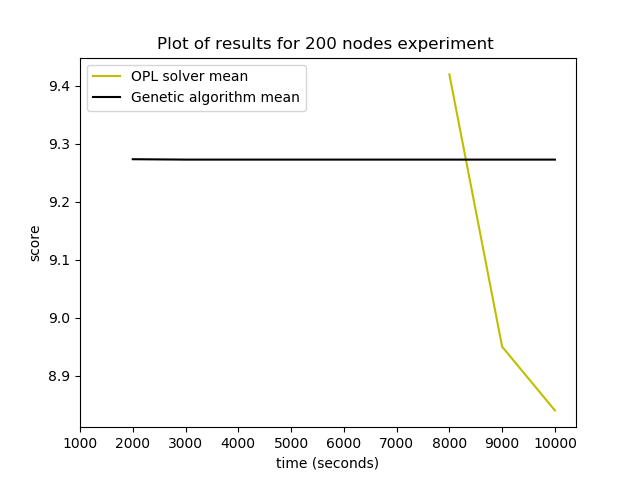
\includegraphics[width=0.6\textwidth]{pics/200_nodes_results.png}
\caption{result of the experiment (single run) on the 200 points dataset}
\label{fig:200points}
\end{figure}

Again, both methods have been restricted with the same stopping criterion, in this case 10000 seconds of computation time. Here the optimal solution hasn't been found by the exact solver within the time constraints, and is therefore not available. \\
Results are presented in figure \ref{fig:200points}. We confirm the trend from the previous experiments, where the exact solver finds a better solution of the genetic algorithm only after a long time. Even more, it is able to find a feasible solution only after about 8000 seconds, while \textit{TSPSolver} is able to find one straight away. On the other hand, with the increase of the search space magnitude we can see that the solution found by the genetic algorithm seems to be more distant from the optimal one, that is instead asymptotically approached by the OPL solver, which reported an estimated gap of $1.89\%$ with the optimal solution.



\section{Conclusions}
This project has been interesting for many reasons: the choice between exact methods and heuristics allows the flexibility of optimizing towards different goals. If one prefers a non optimal solution, but with high speed of implementation and results, heurisitics are a good quick and dirty solution, even if they come with the burden of parameters optimization. The disatvantage though, is that they don't present guarantees of convergence. For this reason in performance critic applications one may prefer to restore to an exact solver, that, even if sometimes in a longer time, converges to the optimum, or is at least able to estimate the gap with respect to it. \\
Overall, I have been able to get acquainted with many tools for combinatorial optimization, and feel confident that in the future I will be able to have a good grip on many problems of this type, thanks to the methods learnt during this course, both on a model and on a solution perspective.




\newpage
\bibliographystyle{ieeetr}
\bibliography{bibliography}
\end{document}